% !TEX root = ../thesis-index.tex


\chapter{Warmup}\label{ch:warmup}

This chapter aims to give an overview and familiarize the reader with the main concepts that are central to this thesis. In that regard, it is written as a self-contained, less rigorous introduction to the main ideas. As the chapters discoveries were made across several years, several ideas were developed, and in fact, similified. Thus, in this chapter, I have the benefit of hindsight to present the ideas in a more coherent and simplified manner than then were originally discovered. 

The central theme of this thesis is stability of forward pass, the form of rank collapse issue, and backward pass, in the form of vanishing or exploding gradients. While stabilising the forward pass is relatively easy using normalization layers, stabilizing the backward pass is more challenging problem. 

\section{Linear MLP: challenges of long tailed distributions}

We begin with a warm-up example of a linear MLP. Let \( x_\ell \in \mathbb{R}^{d_\ell} \) be the activation for layer \( \ell \), where the layers are governed by the following equation:
\begin{equation}
x_\ell = W_\ell x_{\ell-1}, \quad W_\ell \in \mathbb{R}^{d_\ell \times d_{\ell-1}}, \quad x_\ell \in \mathbb{R}^{d_\ell}, \quad \ell = 1, \dots, L,
\end{equation}
where \( W_{\ell} \) is a Gaussian matrix with elements drawn independently from \( N(0,\sigma_\ell^2) \), and the variances \( \sigma_\ell^2 \) are constants. We assume that \( x_0 \in \mathbb{R}^{d_0} \) is our input of dimension \( d_0 \). As mentioned before, our goal is to ensure that the forward and backward activations neither vanish nor explode.

\subsection{Forward Pass Analysis}

\begin{theorem}[Forward Pass Stability]
To ensure the stability of the forward pass, the magnitude of each element of \( x_\ell \), such as its variance, must remain constant. We measure this magnitude using the Root Mean Squared (RMS) norm:
\begin{equation}
\|x\|_{rms} = \sqrt{\frac{1}{d} \sum_{i=1}^d x_i^2}, \quad x \in \mathbb{R}^d,
\end{equation}
which measures the mean magnitude of the elements of a vector. Assuming that \( \|x_0\|_{rms}^2 = 1 \), we try to ensure that \( E\|x_\ell\|_{rms}^2 = 1 \).
\end{theorem}

\begin{proof}
Expanding the activation conditioned on the previous layer, we have \( E[\|W_\ell x_{\ell-1}\|_{rms}^2 | x_{\ell-1}] \), which, using the linearity of expectation, can be simplified to:
\begin{equation}
E \|x_\ell\|_{rms}^2 = \sigma_\ell^2 d_{\ell-1} \|x_{\ell-1}\|_{rms}^2.
\end{equation}
Recursively calculating the norms of previous hidden activations, we obtain \( E \|x_\ell\|_{rms}^2 = \sigma_\ell^2 d_{\ell-1} \cdots \sigma_1^2 d_0 \). If the sequence \( \{\sigma_\ell^2 d_{\ell-1}\}_{\ell=1,\dots,L} \) is even slightly larger or smaller than 1, it will lead to explosion or vanishing values for the norm of \( x_\ell \) as \( \ell \) increases. This observation immediately suggests setting the variance of the Gaussian layer to the inverse of its output dimension \( \sigma_\ell^2 = 1/d_{\ell-1} \), which coincides with the Kaiming initialization \cite{he2015delving}:
\begin{equation}
W_\ell \sim N\left(0, \frac{1}{d_{\ell-1}}\right)^{d_\ell \times d_{\ell-1}} \implies E \|W_\ell \dots W_1 x_0 \|_{rms}^2 = \|x_0\|_{rms}^2,
\end{equation}
meaning that, in expectation, the norm of activations remains similar to the input norm.
\end{proof}

\subsection{Backward Pass Analysis}

\begin{theorem}[Backward Pass Stability]
To ensure the stability of the backward pass, the gradients with respect to a given layer must not vanish or explode. Let \( \mathcal{L}: \mathbb{R}^{d_L} \to \mathbb{R} \) be a loss function that maps the \( L \)-th layer activations to a scalar value. The backward gradients can be computed via the chain rule as follows:
\begin{equation}
\delta_\ell := \frac{\partial \mathcal{L}(x_L)}{\partial x_\ell } = \frac{\partial \mathcal{L}(x_L)}{\partial x_L} W_L \dots W_{\ell+1}, \quad
\frac{\partial x_{\ell+1}}{\partial W_\ell} = x_\ell, \quad
\frac{\partial \mathcal{L}(x_L)}{\partial W_\ell} = \delta_\ell \otimes x_\ell,
\end{equation}
where \( \otimes \) denotes the Hadamard product.
\end{theorem}

\begin{proof}
Expanding \( x_\ell \) and the error vectors \( \delta_\ell \), we set the backward pass to the negative of the gradients:
\begin{equation}
dW_\ell := -\left(\frac{\partial \mathcal{L}(x_L)}{\partial x_L} W_L \dots W_{\ell+1} \right) \otimes \left(W_{\ell-1} \dots W_0 x_0\right).
\end{equation}
Since the Jacobian of each layer equals the weight matrices, the matrix product chain also appears in the backward gradients, which is one of the distinctive features of a linear MLP. Therefore, by setting the variances \( \sigma_\ell \) according to the criteria mentioned earlier, we ensure that the backward gradients are also stable. Assuming the inputs and the gradients with respect to the last hidden layer are of some constant magnitude \( \|x_0\|_{rms}, \|\partial \mathcal{L}(x_L)/\partial x_L\|_{rms} = \Theta(1) \), and using the fact that \( \|u \otimes v\|_F^2 = \|u\|^2 \cdot \|v\|^2 \), we have:
\begin{equation}
\begin{aligned}
E \frac{1}{d_\ell d_{\ell-1}}\|dW_\ell\|_F^2 &= E \|W_{\ell+1}^\top \dots W_L^\top \frac{\partial \mathcal{L}(x_L)}{\partial x_L} \|^2_{rms} \cdot E \|W_{\ell-1} \dots W_0 x_0\|^2_{rms} \\
&= \Theta\left(\frac{1}{d_\ell} E \|W_0 \dots W_{\ell-1}\|_F^2 \frac{1}{d_\ell} E \| W_L \dots W_{\ell+1}\|_F^2\right) \\
&= \Theta(1).
\end{aligned}
\end{equation}
Thus, the backward gradients are also of constant magnitude \( O(1) \). At this point, we might conclude that the problem of stabilizing the forward and backward pass for a linear MLP has essentially been resolved. However, a simulation of this MLP reveals strange and mysterious behavior.
\end{proof}

\section{Long-Tailed Distribution of Activations in Depth}

\begin{remark}
As mentioned earlier, setting the variances of layer \( \ell \) to \( 1/d_{\ell-1} \) ensures that the quantity \( \|x_L\|/\|x_0\| \) is, on average, equal to 1. Let us delve deeper into the distribution of forward activations by plotting \( \|x_L\| \) for random choices of Gaussian weights when the input vector is a uniformly drawn unit vector \( \|x_0\| = 1 \).
\end{remark}

\begin{figure}[H]
    \centering
    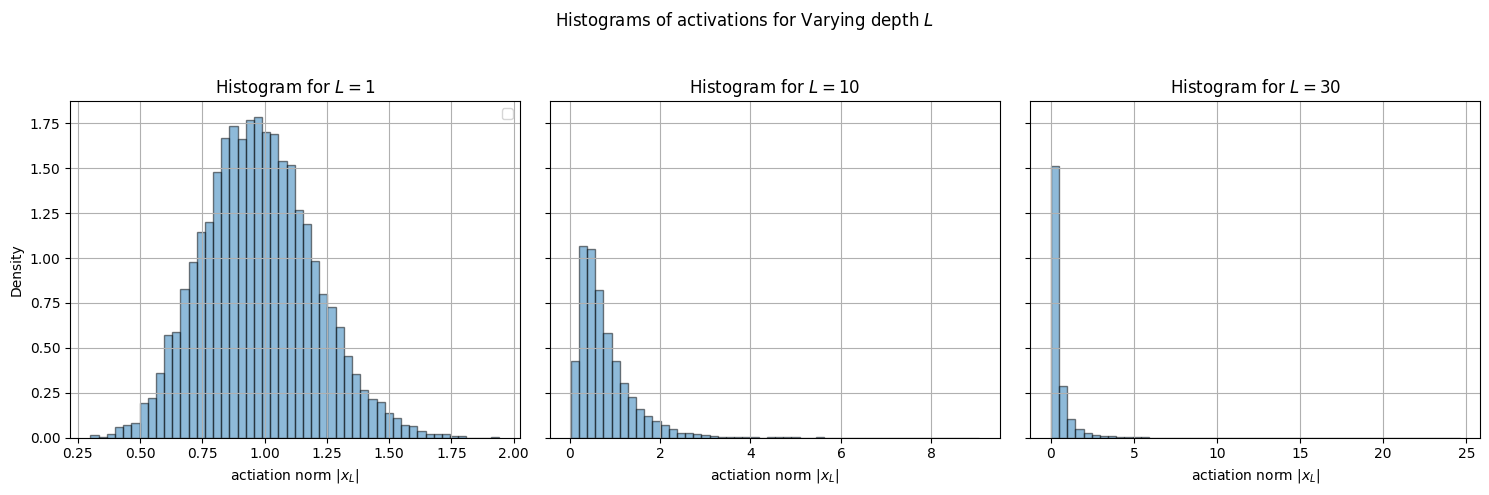
\includegraphics[width=0.8\textwidth]{./MLP_linear_forward_hist.png}
    \caption{Histogram of forward pass activations \( \|x_L\| \) for width \( d=10 \), random choices of Gaussian weights, and a uniformly drawn unit vector as input \( \|x_0\|=1 \). Depth \( L \) is varied to see the effect on the distribution.}
    \label{fig:MLP_hist}
\end{figure}

\begin{remark}
As shown in Figure \ref{fig:MLP_hist}, when the depth is small (\( L=1 \)), the mean calculated earlier predicts the actual values of our activations. However, as the network depth increases, as demonstrated by the subfigure for \( L=20 \), the distribution becomes more heavy-tailed, while the bulk of its values are very small. If we test an even deeper network, such as \( L=100 \), more than half of the values are below 0.01, while in about 1 in every 1000 networks, the value exceeds 10. The mean activation is the average of a few unlikely events where the norm is large (\( >1 \)) and the majority of events where the value is nearly zero.
\end{remark}

In plain words, as the network depth grows, most initialized networks exhibit vanishing activations, while a small number have exploding activations. Therefore, the average behavior for a randomly initialized network is the mean between these two extremes, giving the false impression that forward activations are stable. In statistical terms, the mean value is only predictive for light-tailed symmetric distributions. As the depth grows, the distribution of activations becomes heavy-tailed and highly skewed.

\section{Stabilizing the Forward Pass via Normalization}

\begin{theorem}[Normalization for Stabilizing Forward Activations]
One remedy for stabilizing forward activations is simple normalization, which can be applied on top of our MLP activations to ensure they have constant norms:
\begin{equation}
x_{\ell+1} = W_\ell \tilde{x}_\ell, \quad \tilde{x}_\ell = \frac{x_\ell}{\|x_\ell\|_{rms}}, \quad \ell = 0, \dots, L-1.
\end{equation}
Thus, it will always hold that \( E \|x_L\|^2 = d_L \). However, the additional normalization leads to different behavior between the forward and backward passes.
\end{theorem}

\begin{remark}
This difference stems from a well-known mathematical fact: the product of a chain of Gaussian matrices converges to a rank-1 matrix as the number of these matrices increases \cite{latouche1999introduction}. Consequently, the activations for any two different inputs become increasingly aligned as the depth grows.
\end{remark}

\begin{figure}[H]
    \centering
    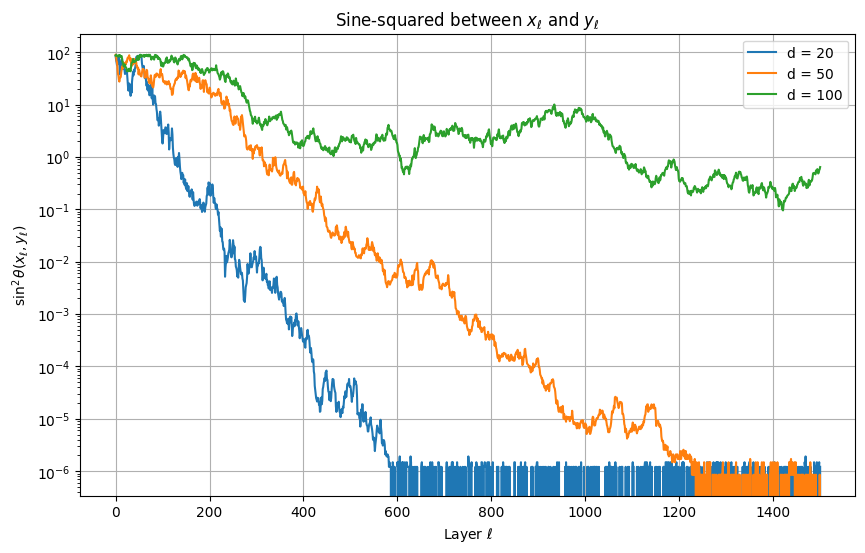
\includegraphics[width=0.8\textwidth]{./lin_MLP_collapse_sine.png}
    \caption{Mode collapse in linear MLP with normalization: for two randomly chosen inputs \( x_0 \) and \( y_0 \), we show the angle between \( x_\ell \) and \( y_\ell \) as measured by \( \sin(\theta_\ell) \). The y-axis shows sine-squared in log-scale, and the x-axis shows depth.}
    \label{fig:MLP_collapse}
\end{figure}

\begin{remark}
As shown in Figure \ref{fig:MLP_collapse}, the y-axis is in log-scale, and the linear decay in sine-squared of the angle implies an exponential convergence of \( \theta \) to 0. Thus, if we vary the weights at layer \( \ell \), the output will only change along one dimension \( W_L \dots W_{\ell+1} dW_\ell \), which is along the direction of the left singular vector of \( W_L \dots W_{\ell+1} \). This issue might seem harmless at first. However, because of the normalization at the very last layer, any changes that affect the norm of the output will be canceled out, leading to vanishing gradients, as evident in Figure \ref{fig:MLP_rank_collapse_vanishing_grads}.
\end{remark}

\begin{figure}[H]
    \centering
    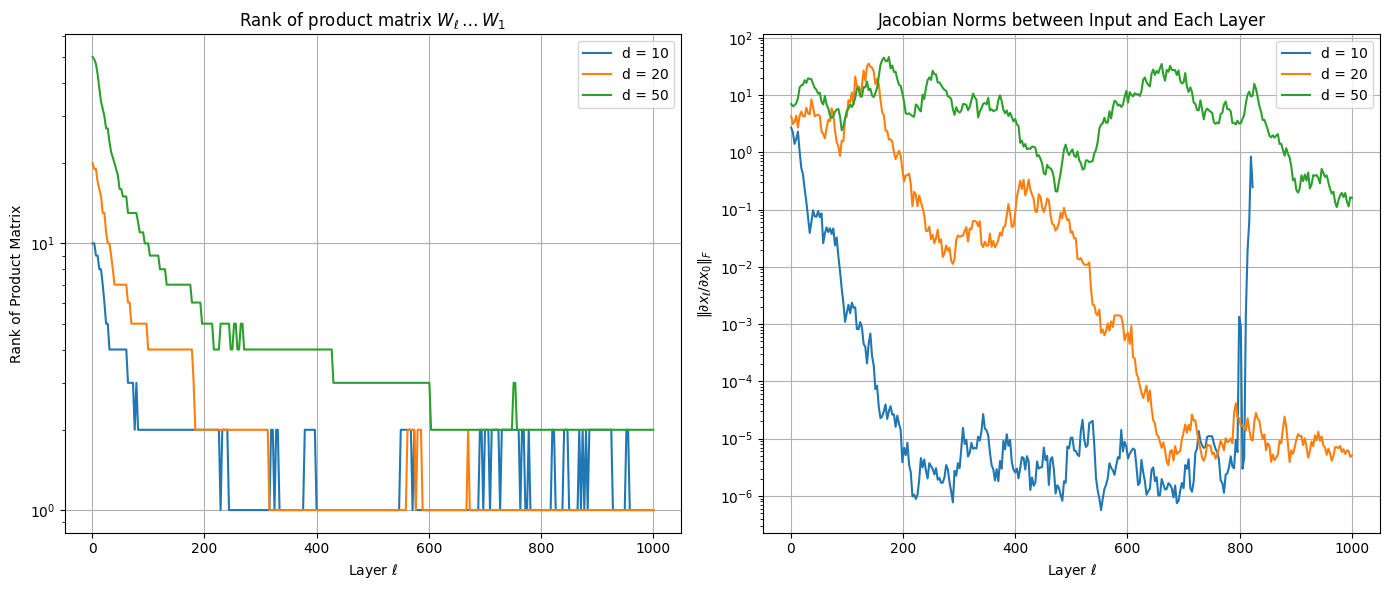
\includegraphics[width=0.8\textwidth]{./rank_collapse_vanishing_grads.png}
    \caption{In MLP with RMS normalization for forward pass, collapse of rank of Jacobian matrix, leads to vanishing gradients.}
    \label{fig:MLP_rank_collapse_vanishing_grads}
\end{figure}

\begin{theorem}[Vanishing Gradients Due to Rank-1 Convergence]
In a linear MLP with normalization layer, if the Jacobian rank collapses to 1, the gradients vanish.
\end{theorem}

\begin{proof}
First, we can ignore all normalization layers except the last one, as adding or removing those normalization constants will not affect the output:
\begin{equation}
\tilde{x}_L = \frac{x_L}{\|\tilde{x}_L\|_{rms}}, \quad x_{\ell+1} = W_\ell x_\ell \quad \ell = 0, \dots, L-1.
\end{equation}
The only difference will be in the introduction of the last normalization layer, which we can focus on analyzing:
\begin{equation}
\tilde{x} := \frac{x}{\|x\|_{rms}} \implies \frac{\partial \tilde{x}}{\partial x} = \frac{1}{\|x\|} \left( I - \frac{1}{d}(x/\|x\|)^{\otimes 2} \right).
\end{equation}
We can focus on understanding \( \partial \tilde{x}_L/\partial x_\ell \). Let \( P := W_L \dots W_0 \) and \( Q := W_L \dots W_{\ell+1} \). We thus have:
\begin{equation}
\begin{aligned}
\frac{\partial \tilde{x}_L}{\partial x_{\ell+1}} &= \frac{\partial \tilde{x}_L}{\partial x_L}\frac{\partial x_L }{\partial x_{\ell+1}} \\
&= \|x_L\|^{-1}_{rms} Q -\frac{1}{d_L}\|x_L\|^{-3}_{rms} x_L x_L^\top Q \\
&= Q / \| P x_0\|_{rms} -  \frac{1}{d} P x_0 x_0^\top P^\top Q / \| P x_0\|^{3}_{rms}.
\end{aligned}
\end{equation}
As the distance between \( \ell \) and \( L \) grows, as shown by \cite{latouche1999introduction}, the product converges to a rank-1 matrix. In the extreme case where \( Q \) is exactly a rank-1 matrix, we can prove that the gradients completely vanish. Assume \( Q = W_L \dots W_{\ell+1} = u v^\top \), where \( u \) and \( v \) are vectors. Since \( P = Q (W_\ell \dots W_0) \), \( P \) is also a rank-1 matrix: \( P = u w^\top \), where \( w = (W_\ell \dots W_0)^\top v \). Let us assume without loss of generality that \( \|u\| = 1 \). Thus, we have:
\begin{equation}
\begin{aligned}
\frac{\partial \tilde{x}_L}{\partial x_{\ell+1}}  
&= u w^\top / \| u v^\top x_0\|_{rms} -  \frac{1}{d} u v^\top x_0 x_0^\top v u^\top  u w^\top / \| u v^\top x_0\|^{3}_{rms} \\
&= u w^\top / (v^\top x_0 /\sqrt{d}) - u ((v^\top x_0)/\sqrt{d})^2 w^\top / ( v^\top x_0/\sqrt{d})^{3} \\
&= u w^\top / (v^\top x_0 /\sqrt{d}) - u w^\top / (v^\top x_0 /\sqrt{d}) \\
&= 0.
\end{aligned}
\end{equation}
If we expand the backward gradients, we have:
\begin{equation}
\frac{\partial \mathcal{L}(x_L)}{\partial W_\ell} = \frac{\mathcal{L}(x_L)}{\partial x_L}\frac{\partial x_L}{\partial \tilde{x}_{\ell+1}}\frac{\partial x_{\ell+1}}{\partial W_\ell} = 0.
\end{equation}
This notion of vanishing gradients can be refined to account for the "distance" to a rank-1 matrix.

Thus, the convergence of the matrix products \( W_L \dots W_{\ell+1} \) to a rank-1 matrix leads to a vanishing gradients problem. This case highlights the importance of analyzing and understanding backward gradients, even when the forward pass is stable. This example illustrates that if we try to normalize the forward pass when the gradients converge to a rank-1 structure, it will lead to a vanishing gradient problem.
\end{proof}


\section{Modeling Long-Tailed Distributions as Geometric Brownian Motion}

\begin{remark}
Many of the emerging phenomena related to matrix products can be viewed through the lens of geometric Brownian motion. In its basic form, geometric Brownian motion models a variable at time \( t \) as \( X_{t} = r_t X_{t-1} \), where \( r_t \) is a log-normal random variable \( \log(r_t) \sim N(\mu, \sigma^2) \), and is used as a simple model to capture price movements at small time scales. Assuming \( X_1=1 \) and taking the logarithm, we have \( \log(X_t) = \log(r_t) + \dots + \log(r_1) \), which is a sum of iid Gaussian variables, and follows \( \log(X_t) \sim N(\mu t, t\sigma^2) \).
\end{remark}

\begin{theorem}[Expected Value of Geometric Brownian Motion]
Using the moment-generating function of the normal distribution, we find that:
\begin{equation}
E[X_t] = E[e^{\log(X_t)}] = \exp(\mu t + \sigma^2 t^2 / 2).
\end{equation}
Thus, even when \( \mu < 0 \), for sufficiently large values of \( \sigma^2 \), the expectation of \( X_t \) can be very large, while \( \log(X_t) \) on average will be a negative value \( \mu t \). This results from the exponential function making the distribution of normal values highly skewed, so its mean value is an average of unlikely large values and likely small values.
\end{theorem}

\begin{remark}
This behavior is analogous to the case of the linear MLP, where the expected forward pass is constant, but in almost all cases, the forward pass is very small. This analogy is not coincidental; there are concrete principles connecting these two examples.
\end{remark}

\subsection{Corollary: Vanishing Norm of Activations}

\begin{corollary}
Let \( W_0, \dots, W_L \) be a set of \( d \times d \) Gaussian matrices with elements drawn from \( N(0, 1/d) \). Suppose \( x_0 \in \mathbb{R}^{d_0} \) is an arbitrary unit vector, \( \|x_0\| = 1 \). Then the norm of activations \( x_\ell = W_\ell \dots W_0 x_0 \) will, in most cases, have a very small value as \( \ell \) grows. Specifically, we have:
\begin{equation}
\lim_{\ell\to\infty} E \left[\log \|x_L\|_{rms}^2\right] = -\sum_{\ell=1}^L \frac{1}{2d_\ell} + o(1),
\end{equation}
where the \( o(1) \) term goes to zero with a rate of \( \sum_{\ell=1}^L 1/d_\ell^2 \).
\end{corollary}

\begin{proof}
We can model the evolution of the length of \( \|x_\ell\| \) as it passes through layers. Let \( W \) be one of the Gaussian layers with an SVD decomposition \( W = \sum_{i=1}^d s_i u_i v_i^\top \), where \( x \) is a non-zero input vector, and \( x' = W x \). We want to understand the distribution of norm-ratios \( \|x'\|^2/\|x\|^2 \). Assuming \( x \) is perfectly parallel to one of the right singular vectors of the weight matrix \( W \), i.e., one of the \( u_i \)'s chosen at random, we approximate the log-ratios by averaging the log-singular values of the weight matrix:
\begin{equation}
\log (\|x'\|^2/\|x\|^2) \approx \frac{1}{d} \sum_{i=1}^d \log(s_i^2(W)).
\end{equation}
Thus, the effect on the \( L \)-th layer will be approximately:
\begin{equation}
\log(\|x_L\|^2/\|x_0\|^2) \approx \sum_{\ell=1}^L \frac{1}{d} \log \det(W_\ell^\top W_\ell).
\end{equation}
Since the expected log-determinant of \( W_\ell^\top W_\ell \), a Wishart matrix, can be calculated in closed form, we have:
\begin{equation}
E\left[\log \det(W^\top W)\right] = n \log(2/d) + \sum_{i=0}^{n-1} \psi\left(\frac{d-i}{2}\right), \quad W \in \mathbb{R}^{d \times n}, W_{ij} \sim N(0, 1/d).
\end{equation}
From this, we conclude:
\begin{equation}
\log(\|x_L\|/\|x_0\|) \approx -\Theta(L),
\end{equation}
leading to the stated corollary.
\end{proof}

\subsection{Corollary: Convergence of Angles between Activations}

\begin{corollary}
Let \( x_0 \) and \( y_0 \) be two randomly chosen input vectors that are orthogonal, and let \( x_\ell \) and \( y_\ell \) denote their corresponding activations at layer \( \ell \). The angle between these representations, measured by \( \sin(\theta_\ell) \), converges as follows:
\begin{equation}
\lim_{\ell\to\infty} E \left[\log \sin(\theta_\ell)^2\right] =  -\sum_{\ell=1}^L \frac{1}{2d_\ell} + O\left(\frac{1}{\sum_{\ell=1}^L d_\ell^2}\right).
\end{equation}
\end{corollary}

\begin{proof}
Form the matrix \( X_\ell \) with \( x_\ell \) and \( y_\ell \) as its first and second columns. Note that \( \det(X_\ell^\top X_\ell) \) can be decomposed into \( \|x_\ell\|^2\|y_\ell\|^2 \cdot (1-\cos(\theta_\ell)^2) \). Thus we can write:
\begin{equation}
\log(1-\cos^2(\theta_\ell)) = \log \det(X_\ell^\top X_\ell) - \log\|x_\ell\|^2 - \log\|y_\ell\|^2.
\end{equation}
Taking expectations and simplifying, we obtain:
\begin{equation}
E \left[\log \sin^2(\theta_\ell)\right] =  -\sum_{\ell=1}^L \frac{1}{2d_\ell} + O\left(\frac{1}{\sum_{\ell=1}^L d_\ell^2}\right).
\end{equation}
\end{proof}

\section{Non-Asymptotic Bounds for Eigenvalues}

\begin{remark}
While the analysis of matrix products has often been conducted in asymptotic regimes, there is a growing demand for non-asymptotic analysis of neural networks due to their relatively small size compared to asymptotic assumptions. Here, we show that the same framework for analyzing log-determinants, or log-average singular values, can be surprisingly easy to convert to non-asymptotic bounds by relying on simple facts such as their sub-exponential behavior.
\end{remark}

\subsection{Corollary: Log-Determinant for Gaussian Matrices}

\begin{corollary}
Let \( W \in \mathbb{R}^{d \times n} \) be a matrix whose rows are drawn iid from \( N(0, \Sigma) \). When \( n/d \) is sufficiently small, the log-determinant of \( W^\top W \) is normally distributed with mean and variance given by:
\begin{equation}
\log \det(W^\top W/d) \to N\left(\log \det \Sigma - \frac{n^2}{2d}, \frac{2n}{d}\right).
\end{equation}
\end{corollary}

\subsection{Corollary 1: Norm Ratio of Linear MLP}

\begin{corollary}
In the setting of a linear MLP, the quantity \( \log(\|x_L\|^2/\|x_0\|^2) \) will be within a \( \sqrt{\sum_{\ell=1}^L\frac{2}{d_\ell}} \)-vicinity of \( -\sum_{\ell=1}^L\frac{1}{2d_\ell} \) with high probability:
\begin{equation}
\log(\|x_L\|^2/\|x_0\|^2) \to N\left(-\sum_{\ell=1}^L \frac{1}{2d_\ell}, \sum_{\ell=1}^L \frac{2}{d_\ell}\right).
\end{equation}
\end{corollary}

\begin{proof}
Let \( x \in \mathbb{R}^{d_1} \) and \( W \) be a \( d_2 \times d_1 \) Gaussian matrix with elements drawn from \( N(0,1/d_1) \). Define \( y = W x \), a \( d_2 \)-dimensional vector whose elements are drawn from \( N(0,\|x\|^2) \). The log-det central limit theorem (CLT) implies:
\begin{equation}
\log(\|y\|^2/d_2) \to N(\log\|x\|^2 - \frac{1}{2d_2}, \frac{2}{d_2}).
\end{equation}
Summing these normal variables across layers \( W_L \dots W_1 x_0 \) yields:
\begin{equation}
\log(\|x_L\|^2/\|x_0\|^2) \to N\left(-\sum_{\ell=1}^L \frac{1}{2d_\ell}, \sum_{\ell=1}^L \frac{2}{d_\ell}\right).
\end{equation}
Thus, \( \log(\|x_L\|^2/\|x_0\|^2) \) will be within a \( \sqrt{\sum_{\ell=1}^L\frac{2}{d_\ell}} \)-vicinity of \( -\sum_{\ell=1}^L \frac{1}{2d_\ell} \) with high probability.
\end{proof}

\subsection{Corollary 2: Angle Between Activations in MLP}

\begin{corollary}
Let \( X_0 \in \mathbb{R}^{d \times 2} \) represent two inputs \( x \) and \( y \), and let \( X_\ell \) denote the activations of these two inputs at various layers of the linear MLP. The angle between two representations in layers obeys the following universality:
\begin{equation}
\log(\sin^2\theta_L/\sin^2\theta_0) \to N\left(-\sum_{\ell=1}^L\frac{1}{d_\ell}, \sum_{\ell=1}^L \frac{8}{d_\ell}\right).
\end{equation}
\end{corollary}

\begin{proof}
Let \( X \) and \( Y = X W \) denote two successive activations where \( W \) is a \( d_1 \times d_2 \) matrix with elements drawn from \( N(0, 1/d_1) \). Each row of \( Y \) is drawn iid from \( N(0, X^\top X) \), and the log-det CLT implies:
\begin{equation}
\log \det(Y^\top Y) \to N(\log \det(X^\top X) - \frac{2}{d_2}, \frac{4}{d_2}).
\end{equation}
Successive application gives:
\begin{equation}
\log \det(X_L^\top X_L) - \log \det(X_0^\top X_0) \to N\left(-\sum_{\ell=1}^L \frac{2}{d_\ell}, \sum_{\ell=1}^L \frac{4}{d_\ell}\right).
\end{equation}
For columns \( x_\ell \) and \( y_\ell \), we obtain:
\begin{equation}
\log \|x_L\|^2 + \log \|y_L\|^2 - (\log \|x_0\|^2 + \log \|y_0\|^2) \to N\left(-\sum_{\ell=1}^L \frac{1}{d_\ell}, \sum_{\ell=1}^L \frac{4}{d_\ell}\right).
\end{equation}
Since \( \det(X_\ell^\top X_\ell) \) can be expressed as \( \det([1 \cos\theta_\ell; \cos\theta_\ell, 1]) \|x_\ell\|^2 \|y_\ell\| \), we have:
\begin{equation}
\log(\sin^2\theta_L/\sin^2\theta_0) \to N\left(-\sum_{\ell=1}^L\frac{1}{d_\ell}, \sum_{\ell=1}^L \frac{8}{d_\ell}\right).
\end{equation}
\end{proof}

\section{Batch Normalization}

\subsection{Big BN Hypothesis}

\begin{theorem}[Big BN Hypothesis]
The behavior of batch normalization (BN) in deep neural networks can be summarized in the following observations:
\begin{enumerate}
    \item If the rank of the input matrix \( X \) is small (say \( r < n \)), the process of fully connected layers plus batch normalization behaves similarly to the case where the batch size is explicitly equal to \( r \). This is because projecting points lying on an \( r \)-dimensional plane in \( \mathbb{R}^n \) onto a sphere is effectively the same as projecting points in the reduced \( r \)-dimensional space onto a sphere, modulo the radius of the sphere. The BN operation cancels out any constant scaling per layer, so this additional scale does not change the per-layer dynamics.
    \item Every small-ish eigenvalue of the Gram matrix \( \lambda_i(X^\top X) \) that is smaller than 1 undergoes an expected improvement in the mean-field regime such that its logarithm improves by \( c/n \) for some constant \( c \). However, due to the limited size \( d \), the log-eigenvalues of the weight matrix covariance are, on average, \( -n/2d \). The convolution of the two implies that small-ish eigenvalues change by \( c/n - n/2d \). If \( d = \Omega(n^2) \), the dynamics of the smallest eigenvalue will be positive until it is no longer small, giving a rate of \( r = c/n - n/2d > 0 \) per layer, and it would take \( O(-\log(\lambda_i(\text{input}))/r) \) layers to bring this eigenvalue to a constant value.
    \item Combining the first two observations, when \( d \) is not sufficiently large and \( r < 0 \), smaller eigenvalues vanish at a rate of \( -\log(\lambda(\text{layer}\ell))\approx r \ell \). Once a sufficient number of eigenvalues vanish, the rank stabilizes at approximately \( \sqrt{d} \), and adding more layers will not significantly change the rank.
\end{enumerate}
\end{theorem}

\subsection{Speculative Refinement}

\begin{remark}
The improvement in the infinite width regime is \( c/n (1-\lambda) \), implying larger eigenvalues have smaller expected improvement, and smaller ones have larger improvement. This induces a stochastic dynamic where smaller eigenvalues grow and larger ones shrink, suggesting that the dynamic is more accurate for the determinant or mean log-eigenvalue.

If we use orthogonal fully connected layers instead of Gaussian layers, the \( -n/2d \) component is absent, which would roughly add \( c/n \) to the log-minimum eigenvalue per layer, or more accurately \( c/n (1-\lambda) \).

When the eigenvalues are sufficiently close to 1, the mean-field dynamics shrink the log-eigenvalues by a constant \( (1-c/n) \) factor, reducing the variance by the same amount. Non-mean-field dynamics add variance of \( n/d \) to the distribution. Thus, the variance of eigenvalues is approximately \( n^2/d \), and their mean is approximately \( -n/d \) at equilibrium.
\end{remark}

\section{Batch Normalization Analysis}

\begin{remark}
Let \( X \) represent a batch normalization operation, where \( X \) is a \( d \times n \) Gaussian matrix with rows drawn iid from \( N(0,\Sigma) \), and \( D \) is a diagonal matrix with \( D_{ii}=1/\|row_i(X)\|_{rms} \). The SVD decomposition of \( DX = D U S V^\top \) leads to:
\begin{equation}
(DX)^\top (DX)  = V^\top S U^\top D^2 U S V.
\end{equation}
Thus, the spectral values are equal to \( U^\top D^2 U (S V^\top S) \), and we have:
\begin{equation}
\log \left[\det\left((DX)^\top (DX)\right)\right] = \log \det(X^\top X) + \log \det\left(U^\top D^2 U\right).
\end{equation}
The first term is simply \( \log \det(X^\top X) \), and the second term is given by the following corollary.
\end{remark}

\subsection{Corollary: Sub-Rotation Log-Determinant}

\begin{corollary}
Suppose \( D \) is a \( d \times d \) matrix, and \( U \) is a random rotation matrix of size \( d \times n \). If \( d \) is divisible by \( n \), then the expected log-determinant of the projection of \( A \) onto the columns of \( U \) is \( n/d \) times the log-volume of \( D \):
\begin{equation}
E \left[\log\left(U^\top D^2 U\right)\right] = \frac{n}{d} \log \det(D^2).
\end{equation}
\end{corollary}

\begin{proof}
If \( d \) is divisible by \( n \), let \( M \in \mathbb{R}^{d \times d} \) be a random rotation matrix. Since \( U \) is a rotation, the spectrum of \( M^\top D \) is equal to the spectrum of \( D \), so \( \det(M^\top D^2 M) = \det(D^2) \).

Let \( M_1, \dots, M_{d/n} \) be the columns packed into \( n \)-sized columns. Since the index of the columns of \( M \) is meaningless, we conclude:
\begin{equation}
E \left[\log\left(M_1^\top D^2 M_1\right)\right] = \frac{n}{d} \log \det(D^2).
\end{equation}
\end{proof}

\section{MLP with Non-Linear Activation}

\begin{remark}
We now extend the analysis to a linear MLP with non-linear activation functions, focusing on the leaky ReLU:
\begin{equation}
f(x) = \begin{cases} x & x \ge 0 \\ \alpha x & x < 0 \end{cases}.
\end{equation}
The forward pass is modeled as \( \log(\|f(W x) \|^2) \), with:
\begin{equation}
\log(\|D W x \|), \quad D_{ii} = diag(f'(x_i))_{i \le n}.
\end{equation}
\end{remark}

\subsection{Lemma: Expected Log-Determinant of Wishart}

\begin{lemma}
If \( W \) is a \( d \times n \) matrix whose elements are drawn iid from \( N(0, 1/d) \), then:
\begin{equation}
E \left[\log \det(W^\top W)\right] = n \log(2) - n \log(d) + \sum_{i=1}^n \psi\left(\frac{d-i+1}{2}\right),
\end{equation}
where \( \psi \) is the digamma function. As an approximation for \( n < d \), we have:
\begin{equation}
E \left[\log \det(W^\top W)\right] = -\frac{n^2}{2d} - \frac{n^3}{6d^2} - \frac{n^4}{3 d^3} + O\left(\frac{n^5}{d^4}\right),
\end{equation}
which becomes more accurate as \( n/d \) decreases.
\end{lemma}

\begin{remark}
Note that the approximation for the normalized log-determinant \( \frac{1}{n} E \left[\log \det(W^\top W)\right] \) depends only on the ratio \( n/d \), meaning the log-determinant, in expectation, does not change if we keep the ratio fixed.
\end{remark}

\begin{proof}
In \cite{braun2010variational}, the authors calculated:
\begin{equation}
\Lambda \sim \mathcal{W}_D(v, \Psi) \implies E \left[\log \det(\Lambda)\right] = D \log(2) + \log\det(\Psi) + \sum_{i=1}^D \psi\left(\frac{\nu-i+1}{2}\right),
\end{equation}
where \( \nu \) is the degrees of freedom, and \( \nu\Psi \) is the mean \( E[\Lambda] = \nu\Psi \). For \( W \) of size \( d \times n \), with \( W_{ij} \sim N(0, 1/d) \), \( E[W^\top W] = I_n \) and it has \( m \) degrees of freedom. So \( \Psi = I_n / d \). Therefore, \( \det(\Psi) = (1/d)^n \implies \log \det(\Psi) = n \log(1/d) \), and thus we have:
\begin{equation}
E \left[\log \det(W^\top W)\right] = n \log(2) - n \log(d) + \sum_{i=1}^n \psi\left(\frac{d-i+1}{2}\right).
\end{equation}
Using the approximation:
\begin{equation}
\psi(z) \approx \log(z) - \frac{1}{2z} - \frac{1}{12 z^2} + \dots,
\end{equation}
and assuming \( d \gg n \), this leads to:
\begin{equation}
E \left[\log \det(W^\top W)\right] \approx -\frac{n^2}{2d} - \frac{n^3}{6d^2} - \frac{n^4}{3d^3} + O\left(\frac{n^5}{d^4}\right).
\end{equation}
For \( n=d \), we have:
\begin{equation}
\frac{1}{d} E \left[\log \det(W^\top W)\right] \approx -1, \quad W \in \mathbb{R}^{d \times d}.
\end{equation}
\end{proof}

\subsection{Central Limit Theorem for Log-Determinant}

\begin{theorem}[CLT for Log-Determinant]
A central limit theorem (CLT) is established for the log-determinant of \( W^\top W \), where \( W \) is a \( d \times n \) matrix with elements drawn iid from \( N(0, 1/d) \) in the high-dimensional setting where the dimension \( n \) grows with the sample size \( d \), with the only restriction that \( n(d) \leq d \). Specifically:
\begin{equation}
\frac{\log \det (W^\top W) - \sum_{i=1}^{d} \log \left(1 - \frac{i}{d}\right)}{\sqrt{-2\log(1-n/d)}} \xrightarrow{distr.} N(0,1) \text{ as } n \to \infty.
\end{equation}
For the boundary case \( n=d \):
\begin{equation}
\frac{\log \det (W^\top W) -\log(n-1)! + n \log n}{\sqrt{2\log n}} \xrightarrow{distr.} N(0,1) \text{ as } n \to \infty.
\end{equation}
\end{theorem}

\begin{remark}
When \( n/d \) is sufficiently small, we have:
\begin{equation}
\log\det(W^\top W) \to N\left(-\frac{n^2}{2d}, \frac{2n}{d}\right).
\end{equation}
For \( n=d \), the distribution is given by:
\begin{equation}
\log\det(W^\top W) \approx N\left(-\log(n-1)! + n \log n, 2\log n\right).
\end{equation}
\end{remark}

\begin{proof}
The result is derived using the central limit theorem for log-determinants of random matrices with iid standard Gaussian entries, as shown in \cite{hazra2019det}. The case when \( n/d \) is small is derived using asymptotic expansions of the digamma function.
\end{proof}
